\documentclass[11pt]{article}
\usepackage[a4paper,margin=25mm]{geometry}
\usepackage{amsmath,amssymb,amsthm,mathtools,booktabs,array,xcolor,graphicx}
\usepackage[T1]{fontenc}\usepackage{lmodern}
\usepackage[colorlinks=true,linkcolor=teal,citecolor=teal,urlcolor=teal]{hyperref}
\hypersetup{pdftitle={Pseudo-Laplacians at Whitney Cross-Caps},pdfauthor={Akari Hayami (Jian-Yu Huang)}}
\graphicspath{{figures/}}
\newtheorem{theorem}{Theorem}[section]
\newtheorem{proposition}[theorem]{Proposition}
\newtheorem{lemma}[theorem]{Lemma}
\newtheorem{corollary}[theorem]{Corollary}
\theoremstyle{definition}\newtheorem{definition}[theorem]{Definition}
\theoremstyle{remark}\newtheorem{remark}[theorem]{Remark}
\newcommand{\R}{\mathbb R}\newcommand{\C}{\mathbb C}\newcommand{\Z}{\mathbb Z}
\newcommand{\Dom}{\operatorname{Dom}}\newcommand{\dd}{\,d}
\newcommand{\norm}[1]{\lVert#1\rVert}
\newcommand{\cH}{\mathcal H}\newcommand{\cV}{\mathcal V}\newcommand{\inte}{\operatorname{int}}
\DeclareMathOperator{\rank}{rank}
\title{Pseudo-Laplacians at Whitney Cross-Caps:\\
Point Interactions on Surfaces Mapped into Three-Space}
\author{Akari Hayami (Jian-Yu Huang)}
\date{October 2026\\\small Version 1}
\setcounter{tocdepth}{1}
\begin{document}\maketitle
\begin{abstract}
On a complete smooth Riemannian surface, Colin de Verdière showed that the Laplacian
restricted to functions vanishing near a point admits a one-parameter family of
self-adjoint extensions, the pseudo-Laplacians, whose domains are described
by a logarithm and a constant. We show that the same picture holds at the
Whitney cross-caps of a surface mapped into $\R^3$. These are the generic
singularities of such maps, and the induced metric degenerates at them.
Each cross-cap carries exactly one logarithmic channel. The leading coefficient
is the universal $-1/(2\pi)$ in the intrinsic distance, or equivalently in the
extrinsic radius, and the regular part is H\"older continuous. With $k$
cross-caps, the extensions of the point-restricted Laplacian are classified by
$U(k)$ in explicit geometric boundary coordinates with a $2\pi$ Green pairing.
The Friedrichs extension is the unique extension with a sub-Markovian
semigroup, and the unique one invariant under change of logarithmic reference
length. The key step is an arclength coordinate that reveals an asymptotically
Euclidean geometry at the cross-cap: the metric is the identity up to
$O(\rho^{1/2})$, which refines Grieser's quasi-isometry of the Whitney umbrella.
Examples include Steiner's Roman surface: its six cross-caps carry a
$U(6)$-family of pseudo-Laplacians, and octahedral symmetry forces its Green
matrix to have at most three eigenvalues.
\end{abstract}
\tableofcontents

\section{Introduction}\label{sec:intro}
Let $X$ be a complete smooth Riemannian surface and $x_0\in X$. Colin de
Verdière \cite{cdv} observed that the Laplacian on $C_c^\infty(X\setminus\{x_0\})$
is not essentially self-adjoint. Its deficiency indices are $(1,1)$, and the
self-adjoint extensions, the \emph{pseudo-Laplacians}, are singled out by the
behaviour
\[
 f(x)=\lambda\Bigl(\sin\alpha\,\tfrac{1}{2\pi}\log r+\cos\alpha\Bigr)+o(1),
 \qquad r=d(x,x_0).
\]
This picture underlies point interactions on manifolds. For conical points
of a flat surface \cite{hk}, the logarithm is again the only channel when the
cone angle is at most $2\pi$; larger angles add power-law channels.

The singularities of a generic smooth map of a surface into $\R^3$, when
present, are isolated \emph{cross-caps} \cite{whitney44,gg}, and they are stable
under small perturbations. At a cross-cap the differential has rank one, and
the induced metric $g=f^*\delta$ degenerates. This paper asks what happens to
point interactions at these points. The answer is pleasantly simple: for the
scalar Laplacian, a cross-cap behaves like a regular point of the surface.
Although the induced metric degenerates there, an arclength coordinate reveals
an asymptotically Euclidean geometry (Lemma~\ref{lem:arclength},
Figure~\ref{fig:umbrella}). This allows the classical logarithmic
point-interaction picture to persist at the singularity, with its exact
coefficient.

\paragraph{Main results.} Let $f:\Sigma\to\R^3$ be a smooth map of a compact
surface, immersive except at finitely many cross-caps; the precise setting is
Definition~\ref{def:setting}. Let $H_F$ be the Friedrichs Laplacian of $g$,
with Dirichlet condition if $\Sigma$ has a boundary, and let $p_1,\dots,p_k$ be
the interior cross-caps.
\begin{enumerate}
\item $H_F$ has compact resolvent (Theorem~\ref{thm:compact}). Every
$u\in\Dom H_F$ is continuous at each $p_j$, and $\tau u=(u(p_j))_j$ is a
graph-bounded surjection onto $\C^k$ with dense kernel
(Theorem~\ref{thm:trace}).
\item The restriction $A=H_F|_{\ker\tau}$ has deficiency indices $(k,k)$, and
its self-adjoint extensions form a $U(k)$-family with explicit Krein resolvent
formula (Theorem~\ref{thm:triple}).
\item Every $\varphi\in\Dom A^*$ has the expansion
$\varphi=\ell_j\log d_g(\cdot,p_j)+b_j+O(d_g^\beta)$ at each $p_j$, and the Green
form is $2\pi(\langle\ell,b'\rangle-\langle b,\ell'\rangle)$. In particular the
resolvent Green vectors have leading term $-\frac1{2\pi}\log d_g$
(Theorems~\ref{thm:log} and~\ref{thm:boundary}).
\item $H_F$ is the only extension with a sub-Markovian semigroup, and the only
one invariant under a common change of logarithmic reference length.
Coefficients on the two sheets meeting at a cross-cap agree in the limit
(Section~\ref{sec:uniqueness}).
\end{enumerate}
Each cross-cap therefore carries one channel, as a regular point does, and
its Whitney invariants enter only through the regular part
(Table~\ref{tab:channels}). The geometric input is the arclength coordinate of
Lemma~\ref{lem:arclength}, in which the metric equals the identity up to
$O(\rho^{1/2})$. This refines Grieser's quasi-isometry of the Whitney umbrella
with the plane \cite{grieser} from bounded distortion to asymptotic equality,
and it is this step that fixes the exact coefficient $-1/(2\pi)$.

\begin{table}[t]\centering\small\renewcommand{\arraystretch}{1.3}
\begin{tabular}{@{}>{\raggedright\arraybackslash}p{.30\linewidth}>{\raggedright\arraybackslash}p{.14\linewidth}>{\raggedright\arraybackslash}p{.36\linewidth}l@{}}\toprule
Point & Total angle & Singular channels at the point & Source\\\midrule
Regular point of a complete smooth surface & $2\pi$ & $\log r$ & \cite{cdv}\\
Conical point of a flat surface & $\theta\leq2\pi$ & $\log r$ & \cite{hk}\\
Conical point of a flat surface & $\theta>2\pi$ & $\log r$ and $r^{-|\nu|}e^{i\nu\phi}$, $\nu=2\pi j/\theta$, $0<|j|<\theta/2\pi$ & \cite{hk}\\
Whitney cross-cap & $2\pi$ & $\log r$ & this paper\\\bottomrule
\end{tabular}
\caption{Singular channels of the point-restricted Laplacian. At a cross-cap
the total angle is $2\pi$ (Remark~\ref{rem:angle}), and a single logarithmic
channel appears, exactly as at a regular point.}\label{tab:channels}
\end{table}

The theory is local at the cross-caps but needs a global boundary condition.
If one instead closes the Laplacian on functions compactly supported in the
interior, every regular boundary arc contributes infinitely many deficiency
modes. The Krein extension of that closure then has an infinite-dimensional
kernel, while its nonzero spectrum is still discrete and is given by a
buckling problem (Section~\ref{sec:boundary}). The examples in Section~\ref{sec:examples}
are Steiner's Roman surface, a closed surface with six cross-caps, and a ruled
surface from an earlier signal model, which also has cross-caps on its boundary.

\paragraph{Relation to the literature.} The abstract extension theory is
Posilicano's \cite{pos}, and the scalar regularity input is the
De Giorgi--Nash--Moser theory in the form of \cite{simon}. Colin de Verdière
\cite{cdv} treats regular points of smooth surfaces and Hillairet--Kokotov
\cite{hk} conical points. Grieser \cite{grieser} supplies the quasi-isometric
coordinates. The contribution here is to carry this circle of ideas to the
generic singular points of surfaces in $\R^3$, together with the sharpened
local geometry that this requires.

\section{Setting}\label{sec:setting}
\begin{definition}\label{def:setting}
Let $\Sigma$ be a compact connected smooth surface, either closed or with a
piecewise smooth Lipschitz boundary, and let $f:\Sigma\to\R^3$ be smooth up to
the boundary. Assume that $f$ is an immersion except on a finite set
$Z\cup Z_\partial$, where $Z\subset\inte\Sigma$ and $Z_\partial\subset\partial\Sigma$,
and that every point of $Z\cup Z_\partial$ is a \emph{Whitney cross-cap} of $f$, or of
a smooth extension of $f$ near $\partial\Sigma$. That is, $df$ has rank one there,
and for a kernel vector $\eta$ and a complementary vector $\xi$,
\begin{equation}\label{eq:whitney}
 \det\bigl(f_\xi,\,f_{\xi\eta},\,f_{\eta\eta}\bigr)\neq0.
\end{equation}
At each $p\in Z_\partial$ we assume that, in some smooth chart of the extension
centred at $p$, $\Sigma$ is a closed sector $\{\theta_1\leq\theta\leq\theta_2\}$.
We write $Z=\{p_1,\dots,p_k\}$. There are two regimes:
\begin{itemize}
\item[(D)] $\partial\Sigma\neq\emptyset$, with the Dirichlet condition imposed
on the whole boundary;
\item[(N)] $\Sigma$ is closed, in which case $Z_\partial=\emptyset$.
\end{itemize}
\end{definition}

The condition \eqref{eq:whitney} is the standard recognition criterion for
the cross-cap $(x,y)\mapsto(x,xy,y^2)$ \cite{hasegawa}. A theorem of Whitney
\cite{whitney44}, see also \cite{gg}, states that the cross-cap is the only
stable singularity of maps from surfaces to $\R^3$. Consequently, for a
generic map the hypotheses hold with $Z_\partial=\emptyset$.

Put $g=f^*\delta$ on $\Sigma\setminus(Z\cup Z_\partial)$. Let $\cH=L^2(\Sigma,dA_g)$
and $q(u,v)=\int\langle\nabla u,\nabla v\rangle_g\dd A_g$. Take as core
$\mathcal C=C_c^\infty(\inte\Sigma\setminus Z)$ in case (D), and the smooth
functions on $\Sigma$ vanishing near $Z$ in case (N). The closure $\cV$ of
$\mathcal C$ in the norm $(q(u,u)+\norm u^2)^{1/2}$ defines a closed form, and
we let $H_F$ be its self-adjoint operator. Scalar products are
conjugate-linear in the first slot.

All operators act on the source. Functions live on $\Sigma$, and $f$ enters only
through the pulled-back metric $g$, its area form and its gradient. Where
$f(s)=f(s')$ for distinct source points, as along the double curves of the Roman
surface, the two points remain distinct, and a function may take different
values on the two sheets. Thus ``the Laplacian of the Roman surface'' means the
Laplacian of $(\mathbb{RP}^2,f^*\delta)$. The self-intersections of the image
play no role; the cross-caps, where $g$ degenerates, are what matter.

\section{Local geometry at a cross-cap}\label{sec:local}
\begin{lemma}[Adapted form]\label{lem:adapted}
After a translation and a rotation of $\R^3$ and a smooth change of source
coordinates centred at a cross-cap, $f(x,y)=(x,h(x,y))$ with $h(0)=0$,
$Dh(0)=0$ and
\[
 h_y(x,y)=xv+2yw+O(R^2),\qquad R=(x^2+y^2)^{1/2},
\]
where $v,w\in\R^2$ are linearly independent. Hence $cR\leq|h_y|\leq CR$ and
$|h_x|\leq CR$. In any smooth chart centred at the point, $g\leq CI$ and
$cR^2\leq\det g\leq CR^2$; in particular $dA_g\asymp R\dd x\dd y$.
\end{lemma}
\begin{proof}
Rotate so that $f_\xi(0)$ points along the first axis. Use $x$, the first
component of $f$, together with any coordinate $y$ completing it to a chart.
Since the image of $df(0)$ is the first axis, $\ker dx(0)=\ker df(0)$, so
$\partial_y$ is a kernel vector at $0$. Then $h_x(0)=0$ and $h_y(0)=0$. The vectors $v=h_{xy}(0)$ and $2w=h_{yy}(0)$
are independent by \eqref{eq:whitney}. In these coordinates
$g=\bigl(\begin{smallmatrix}1+|h_x|^2&h_x\cdot h_y\\h_x\cdot h_y&|h_y|^2\end{smallmatrix}\bigr)$,
whose entries are bounded and whose determinant lies between $|h_y|^2$ and
$(1+|h_x|^2)|h_y|^2$. A smooth change of chart has bounded derivative and
inverse, so these bounds persist.
\end{proof}

\begin{lemma}[Arclength coordinate]\label{lem:arclength}
In the coordinates of Lemma~\ref{lem:adapted} put
\[
 V(x,y)=\int_0^y|h_y(x,s)|\dd s,\qquad \Xi(x,y)=(x,V),\qquad
 \rho=|\Xi|.
\]
Then $\Xi$ is a homeomorphism of a neighbourhood of $0$ onto a neighbourhood
of $0$, and a $C^1$ diffeomorphism off $0$. In the coordinates $(X,V)=\Xi$,
the metric $G$, the density $m=\sqrt{\det G}$ and the divergence tensor
$a=mG^{-1}$ satisfy
\[
 G-I=O(\rho^{1/2}),\qquad a-I=O(\rho^{1/2}),\qquad m-1=O(\rho),
\]
and are bounded and uniformly elliptic. The extrinsic radius
$\rho_e=|f-f(0)|$ satisfies $\rho_e/\rho=1+O(\rho^{1/2})$.
\end{lemma}
\begin{proof}
For fixed $x$, $V$ is strictly increasing in $y$, and
$cy^2\leq|V|\leq C(|xy|+y^2)$. Its inverse is therefore continuous, also at
zero. Differentiating under the integral, with $n=h_y/|h_y|$, gives
$V_y=|h_y|$ and $V_x=\int_0^yn\cdot h_{xy}\dd s$, so $|V_x|\leq C|y|$. Both are
continuous, and $V_y>0$ off zero. In the new coordinates $f_X=(1,q)$ and
$f_V=(0,n)$, where $q=h_x-V_xn$, so
\[
 G=\begin{pmatrix}1+|q|^2&q\cdot n\\q\cdot n&1\end{pmatrix},\qquad
 \det G=1+|q|^2-(q\cdot n)^2\geq1.
\]
Since $|q|\leq CR$ and $R^2\leq C\rho$, the stated bounds follow.

For the radii, Taylor's formula gives $|h-wy^2|\leq C(x^2+|xy|+|y|R^2)$.
Integrating $\bigl||h_y(x,s)|-2|w||s|\bigr|\leq C(|x|+x^2+s^2)$ gives
$\bigl|V-\operatorname{sgn}(y)|w|y^2\bigr|\leq C(|xy|+|y|R^2)$. Hence
$\bigl||h|-|V|\bigr|\leq CR\rho$, and comparing the norms of $(x,|h|)$ and
$(x,|V|)$ gives $|\rho_e-\rho|\leq CR\rho\leq C\rho^{3/2}$.
\end{proof}

\begin{remark}[The standard cross-cap]\label{rem:standard}
For $f(x,y)=(x,xy,y^2)$ one has $h_y=(x,2y)$, and the arclength coordinate is
explicit:
\[
 V(x,y)=\frac y2\sqrt{x^2+4y^2}+\frac{x^2}4\operatorname{arsinh}\frac{2y}{|x|},
 \qquad V(0,y)=y|y|.
\]
Along the double ray $x=0$, $V$ is the signed arclength of the parabola
$y\mapsto(0,0,y^2)$, so the two sheets meeting there are unfolded in opposite
directions (Figure~\ref{fig:umbrella}). Here the general bound improves. With
$q$ and $n$ as in the proof of Lemma~\ref{lem:arclength},
\[
 V_x=\frac x2\operatorname{arsinh}\frac{2y}{|x|},\qquad
 q\cdot n=\frac x2\Bigl(\frac{2y}{\sqrt{x^2+4y^2}}-\operatorname{arsinh}\frac{2y}{|x|}\Bigr),\qquad
 |q|\leq2|y|.
\]
Since $|x|\leq\rho$, $y^2\leq|V|\leq\rho$, and $x\mapsto x\operatorname{arsinh}(a/x)$
is increasing on $(0,\infty)$ for $a>0$, we get
$|x|\operatorname{arsinh}(2|y|/|x|)\leq\rho\operatorname{arsinh}(2\rho^{-1/2})=O(\rho\log(1/\rho))$.
Hence $|q\cdot n|=O(\rho\log(1/\rho))$ and $|q|^2\leq4\rho$, so
$G-I=O(\rho\log(1/\rho))$ for the standard germ. The radii improve in the same
way. Both radii are even in $y$, so take $y\geq0$. With
$A=\operatorname{arsinh}(2y/|x|)$, a direct expansion gives
\[
 V^2-y^4-x^2y^2=-\tfrac34x^2y^2+\tfrac14x^2y\sqrt{x^2+4y^2}\,A+\tfrac1{16}x^4A^2 .
\]
Each term is $O(\rho^3\log(1/\rho))$, and $\rho_e^2-\rho^2=x^2y^2+y^4-V^2$, so
$|\rho_e-\rho|\leq|\rho_e^2-\rho^2|/\rho$ gives $\rho_e/\rho=1+O(\rho\log(1/\rho))$.
Figure~\ref{fig:euclidean} shows both rates numerically.
\end{remark}

\begin{figure}[t]\centering
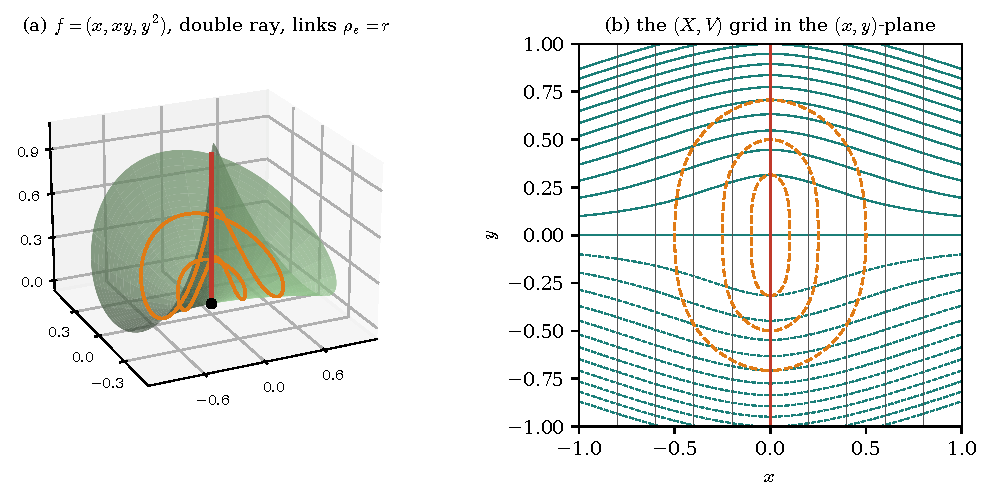
\includegraphics[width=\linewidth]{umbrella_coordinates.pdf}
\caption{(a) The standard cross-cap $f(x,y)=(x,xy,y^2)$ on the unit disc of
the source. The two sheets cross along the double ray (red), which ends at the
cross-cap (black). The orange curves are links $\rho_e=r$, each the image of a
circle with one double point. (b) The arclength coordinate grid of
Remark~\ref{rem:standard}, pulled back to the original $(x,y)$-plane: level
curves of $V$ (teal, dashed where $V<0$) and of $X=x$ (grey). The orange curves
are the preimages of the circles $\rho=0.1,0.25,0.5$ of the $(X,V)$-plane,
which is why they are not round. In the coordinates $(X,V)$ the degenerate
metric becomes asymptotically Euclidean.}\label{fig:umbrella}
\end{figure}

\begin{figure}[t]\centering
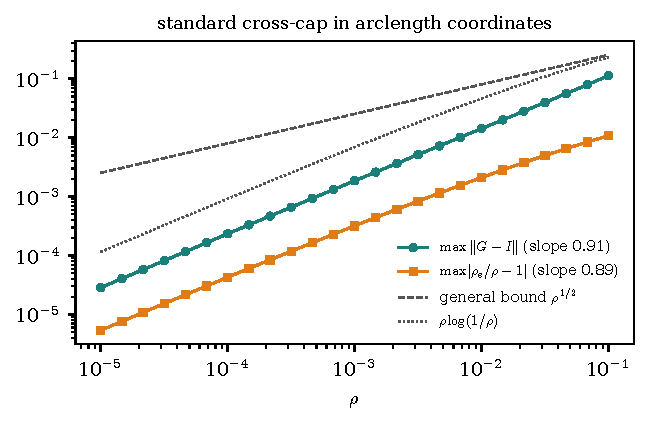
\includegraphics[width=.66\linewidth]{asymptotically_euclidean.pdf}
\caption{Deviation from Euclidean geometry at the standard cross-cap, sampled
at $720$ points of each circle $\rho=r$ in arclength coordinates. Both the
metric deviation $\|G-I\|$ and the radius ratio $\rho_e/\rho$ decay like
$\rho\log(1/\rho)$, the bound of Remark~\ref{rem:standard}, well inside the
general bound $\rho^{1/2}$ of Lemma~\ref{lem:arclength}. The fitted slopes are
least-squares fits over the shaded interval $10^{-5}\leq\rho\leq10^{-3}$. They
are not new exponents: they match the local slope $1-1/\log(1/\rho)$ of
$\rho\log(1/\rho)$, which lies between $0.86$ and $0.91$ there.}\label{fig:euclidean}
\end{figure}

\begin{corollary}[Intrinsic distance]\label{cor:distance}
Let $d_g$ be the path distance of $g$ on the source. Near a cross-cap $p$,
\[
 d_g(\cdot,p)=\rho\bigl(1+O(\rho^{1/2})\bigr),\qquad
 \log d_g(\cdot,p)-\log\rho_e=O(\rho^{1/2}).
\]
\end{corollary}
\begin{proof}
In the arclength coordinates, $|v|^2(1-C\rho^{1/2})\leq v^TGv\leq|v|^2(1+C\rho^{1/2})$.
The straight segment to a point at radius $\rho$ has length at most
$\rho(1+C\rho^{1/2})$. A curve from $p$ to that point either stays in the disk
of radius $2\rho$, and then has length at least $\rho(1-C\rho^{1/2})$, or
crosses the annulus $\rho\leq|\cdot|\leq2\rho$, which costs at least
$\rho(1-C\rho^{1/2})$. Lemma~\ref{lem:arclength} compares $\rho$ with $\rho_e$.
\end{proof}

\begin{remark}
Grieser proved that the Whitney umbrella metric is quasi-isometric to the
Euclidean plane through a singular coordinate change \cite[\S1]{grieser}.
Lemma~\ref{lem:arclength} sharpens this from bounded distortion to
$G=I+O(\rho^{1/2})$. Bounded distortion would suffice for continuity of
point values, but the exact constant $-1/(2\pi)$ requires the sharper form.
\end{remark}

\section{The Friedrichs Laplacian}\label{sec:friedrichs}
\begin{proposition}[Zero capacity]\label{prop:capacity}
Each interior cross-cap has zero capacity for $q$. Consequently $\cV$ is also
the closure of $C_c^\infty(\inte\Sigma)$ in case (D), or of $C^\infty(\Sigma)$ in
case (N).
\end{proposition}
\begin{proof}
In the arclength coordinates, $q$ and the $L^2$ norm on a small disk are
equivalent to the Euclidean $H^1$ and $L^2$ norms. Cutoffs equal to
$\log(\varepsilon/\rho)/\log(1/\varepsilon)$ for $\varepsilon^2\leq\rho\leq\varepsilon$,
suitably smoothed, have Euclidean Dirichlet energy $O(1/\log(1/\varepsilon))$.
Multiplying a smooth function by one minus such a cutoff therefore
approximates it in the form norm by functions vanishing near the point. Smooth
source functions have finite energy, because $|\nabla u|_g^2\dd A_g=O(R^{-1})\dd x\dd y$
by Lemma~\ref{lem:adapted}.
\end{proof}

\begin{theorem}[Compactness]\label{thm:compact}
The embedding $\cV\hookrightarrow\cH$ is compact, so $H_F$ has compact
resolvent. In case (D), $H_F\geq\lambda_D>0$. In case (N),
$\ker H_F$ consists of the constants.
\end{theorem}
\begin{proof}
Fix $p\in Z\cup Z_\partial$ and chart coordinates in which a neighbourhood of
$p$ in $\Sigma$ is a sector: the full disk for interior points, and the sector
of Definition~\ref{def:setting} for boundary points. Let $\chi$ be a
chart cutoff, equal to $1$ near $p$, and let $u\in\mathcal C$, so that $h=\chi u$
vanishes near $p$. On each ray, integrating $(R|h|^2)'$ and applying
Cauchy--Schwarz gives
\[
 \int_0^{R_0}|h|^2\dd R\leq4\int_0^{R_0}R^2|\partial_Rh|^2\dd R .
\]
Integrating over the angular interval and using Lemma~\ref{lem:adapted}
($dA_g\asymp R\dd x\dd y$ and $g\leq CI$),
\[
 \int\frac{|h|^2}{R^2}\dd A_g\leq C\int R|\nabla h|^2\dd x\dd y\leq C'\bigl(q(u,u)+\norm u^2\bigr).
\]
This extends to $\cV$ by closure. Hence the $L^2$ mass in $\{R<\varepsilon\}$ is
at most $C\varepsilon^2$ times the form norm, uniformly over the finitely many
singular points. On the complement of these small sectors, $g$ is a smooth
Riemannian metric on a compact Lipschitz domain, where Rellich's theorem
applies. A diagonal argument together with the uniform small-sector bound gives
compactness.

If $q(u_n,u_n)\to0$ with $\norm{u_n}=1$, a subsequence converges in $\cH$ to a
function with zero gradient on the connected regular locus, which is a
constant. In case (D) its Dirichlet trace on a regular boundary arc vanishes,
so the constant is zero, a contradiction. In case (N) the constants lie in
$\cV$ and form the kernel.
\end{proof}

\section{Point values and the extension problem}\label{sec:extension}
\begin{theorem}[Point traces]\label{thm:trace}
Each $u\in\Dom H_F$ has a unique representative that is continuous at every
$p_j$, H\"older continuous in the arclength coordinates. The map
$\tau u=(u(p_1),\dots,u(p_k))$ satisfies
$|\tau u|\leq C(\norm u+\norm{H_Fu})$, is onto $\C^k$, and has kernel dense
in $\cH$.
\end{theorem}
\begin{proof}
Near $p_j$, in the arclength coordinates, $u$ is a local $H^1$ weak solution
of $-\operatorname{div}(a\nabla u)=m\,H_Fu$. This equation holds across the
point because, by Proposition~\ref{prop:capacity}, test functions vanishing
near the point are dense in $H^1$. The coefficients are real, bounded and
uniformly elliptic, and $m\,H_Fu\in L^2$ with $2>\dim/2$, so the interior
H\"older estimate \cite[Thm.~8.24]{gt}, \cite[Lect.~18]{simon} gives
$\norm u_{C^\alpha}\leq C(\norm u_{L^2}+\norm{H_Fu}_{L^2})$ on a smaller disk.
A cutoff $\chi_j$ equal to $1$ near $p_j$, supported away from the other
singular points and from $\partial\Sigma$, has $\Delta_g\chi_j$ smooth and
supported on a regular annulus, so $\chi_j\in\Dom H_F$ and $\tau\chi_j=e_j$.
Finally the core $\mathcal C$ consists of smooth functions vanishing near $Z$
(and near $\partial\Sigma$ in case (D)); integration by parts on the regular locus
puts it in $\Dom H_F\cap\ker\tau$, and it is dense in $\cH$.
\end{proof}

\begin{theorem}[The point-restricted Laplacian]\label{thm:triple}
The operator $A=H_F|_{\ker\tau}$ is closed, densely defined and symmetric, with
deficiency indices $(k,k)$, and its Friedrichs extension is $H_F$. Fix
$\eta<0$, let $R_z=(H_F-z)^{-1}$, and put $G_z=(\tau R_{\bar z})^*:\C^k\to\cH$.
Then
\[
 \Dom A^*=\Dom H_F\dotplus G_\eta\C^k,\qquad A^*(u+G_\eta a)=H_Fu+\eta G_\eta a.
\]
The maps $\Gamma_0(u+G_\eta a)=a$ and $\Gamma_1(u+G_\eta a)=\tau u$ form a
boundary triple. The self-adjoint extensions are exactly the operators
$(U-I)\Gamma_1+i(U+I)\Gamma_0=0$, $U\in U(k)$, and their resolvents differ from
$R_z$ by operators of rank at most $k$. All of them have compact resolvent. In
case (D), the Krein--von Neumann extension has domain
$\Dom A\dotplus G_0\C^k$ and kernel of dimension $k$.
\end{theorem}
\begin{proof}
Graph continuity makes $\ker\tau$ graph-closed. For nonreal $z$, the bounded
surjection $\tau R_z:\cH\to\C^k$ has kernel $\operatorname{ran}(A-z)$, so
$\dim\ker(A^*-\bar z)=k$. The form core $\mathcal C$ lies in $\Dom A$, so the
Friedrichs extension of $A$ is $H_F$. For $\varphi\in\Dom A^*$, the vector
$u=R_\eta(A^*-\eta)\varphi$ lies in $\Dom H_F$, and $\varphi-u$ lies in
$\ker(A^*-\eta)=\operatorname{ran}(A-\eta)^\perp=G_\eta\C^k$; the sum is direct
because $\eta\in\rho(H_F)$. The Green identity
\[
 \langle A^*\varphi,\psi\rangle-\langle \varphi,A^*\psi\rangle
 =\langle\Gamma_1\varphi,\Gamma_0\psi\rangle-\langle\Gamma_0\varphi,\Gamma_1\psi\rangle
\]
follow from $\langle(H_F-\eta)u,G_\eta b\rangle=\langle\tau u,b\rangle$. This is
the framework of \cite{pos}. Resolvent differences have range in
$\ker(A^*-z)$, which has dimension $k$, and $R_z$ is compact. In case (D) $A$
is strictly positive, and the Krein theorem \cite[Thm.~2.1]{krein} gives
$\Dom A_K=\Dom A\dotplus\ker A^*$, with $\ker A^*=G_0\C^k$ since $0\in\rho(H_F)$.
\end{proof}

\begin{corollary}[Eigenvalue counting]\label{cor:counting}
Every self-adjoint extension $H$ of $A$ is bounded below and has compact
resolvent. Its eigenvalue counting function satisfies
$|N_H(\lambda)-N_{H_F}(\lambda)|\leq k$ for all real $\lambda$.
\end{corollary}
\begin{proof}
Extensions of a semibounded symmetric operator with finite deficiency indices
are semibounded. Choose $\mu$ below both spectra. Then $(H-\mu)^{-1}$ and
$(H_F-\mu)^{-1}$ are positive compact operators whose difference has rank at
most $k$. By Weyl's interlacing inequalities, their eigenvalue counting
functions above any threshold differ by at most $k$. The map
$\lambda\mapsto(\lambda-\mu)^{-1}$ is decreasing on $(\mu,\infty)$, which
transfers the bound to $N_H$ and $N_{H_F}$.
\end{proof}

\section{Logarithmic normalization}\label{sec:log}
\begin{theorem}[Green vectors]\label{thm:log}
For real $\eta<0$ there are $\beta>0$ and a real symmetric matrix $B_\eta$ such
that, near each $p_i$,
\[
 G_{\eta,j}=-\frac{\delta_{ij}}{2\pi}\log d_g(\cdot,p_i)+(B_\eta)_{ij}+O\bigl(d_g(\cdot,p_i)^\beta\bigr).
\]
The same holds with $d_g$ replaced by the extrinsic radius
$\rho_{e,i}=|f-f(p_i)|$, with the same matrix $B_\eta$.
\end{theorem}
\begin{proof}
Fix $i$ and work in arclength coordinates $X$ on a disc $B_{2r_0}$ about $p_i$,
with $r_0$ so small that these discs are disjoint for different poles. There
$\rho=|X|$, $dA_g=m\dd X$, $q(u,v)=\int a\nabla\bar u\cdot\nabla v\dd X$, and
$E=a-I$ satisfies $|E|\leq C\rho^{1/2}$ by Lemma~\ref{lem:arclength}. Since $q$
and $\eta$ are real, $H_F$ commutes with complex conjugation, and it suffices
to pair with real functions.

\emph{Step 1: a parametrix.} Let $\chi$ be a radial cutoff equal to $1$ on
$B_{r_0}$ and supported in $B_{2r_0}$, and put $h_0=-\chi\log\rho/(2\pi)$. Then
$-\Delta h_0=\delta_0+k_0$, with $k_0$ bounded and supported in the annulus
$r_0\leq\rho\leq2r_0$. For $\varphi\in\cV$ put
\[
 \mathcal F(\varphi)=\int E\nabla h_0\cdot\nabla\varphi\dd X+\int(k_0-\eta mh_0)\varphi\dd X .
\]
Since $|E\nabla h_0|\leq C\rho^{-1/2}$, the first density lies in $L^3$, and
$k_0-\eta mh_0$ lies in $L^2$. By uniform ellipticity $\mathcal F$ is bounded on
$\cV$. The form $q_\eta=q-\eta\langle\cdot,\cdot\rangle$ is coercive, so
Lax--Milgram gives a real $w\in\cV$ with $q_\eta(w,\varphi)=\mathcal F(\varphi)$
for all $\varphi\in\cV$. Locally, $w$ solves a uniformly elliptic equation with
divergence data in $L^3$ and scalar data in $L^2$, so the H\"older estimate
\cite[Thm.~8.24]{gt}, \cite[Lect.~18]{simon} makes $w$ H\"older continuous near
every pole. Put $g_i=h_0-w$.

\emph{Step 2: an annulus estimate.} Let $u\in\Dom H_F$ be real. By
Theorem~\ref{thm:trace}, $|u-u(p_i)|\leq C\rho^\alpha$ on $B_{r_0}$. Testing
$-\operatorname{div}(a\nabla u)=m\,H_Fu$ with $\zeta^2(u-u(p_i))$, where $\zeta$
equals $1$ on $B_r$, is supported in $B_{2r}$ and has $|\nabla\zeta|\leq C/r$,
gives the Caccioppoli bound
\[
 \int_{B_r}|\nabla u|^2\leq\frac C{r^2}\int_{B_{2r}}|u-u(p_i)|^2
 +C\int_{B_{2r}}|H_Fu|\,|u-u(p_i)|\leq Cr^{2\alpha}.
\]
On an annulus $A_r=B_{2r}\setminus B_r$ we have $|\nabla h_0|\leq C/r$ and
$|A_r|\leq Cr^2$, so Cauchy--Schwarz gives
$\int_{A_r}|\nabla h_0|\,|\nabla u|\leq Cr^\alpha$. Summing over dyadic annuli
shows that $\nabla h_0\cdot\nabla u$ is integrable on $B_{r_0}$. Now let
$\zeta_\varepsilon$ be radial, equal to $0$ on $B_\varepsilon$ and to $1$ off
$B_{2\varepsilon}$, with $|\nabla\zeta_\varepsilon|\leq C/\varepsilon$. The same
bounds give
\[
 \int|h_0|\,|\nabla\zeta_\varepsilon|\,|\nabla u|\leq C\varepsilon^\alpha|\log\varepsilon|,\qquad
 \int|u-u(p_i)|\,|\nabla h_0|\,|\nabla\zeta_\varepsilon|\leq C\varepsilon^\alpha .
\]
Both tend to zero: excising a small disc costs nothing in the limit.

\emph{Step 3: identification.} Put $v=(H_F-\eta)u$. Since $\zeta_\varepsilon h_0\in\cV$,
\[
 \langle\zeta_\varepsilon h_0,v\rangle=q_\eta(\zeta_\varepsilon h_0,u)
 =\int a\nabla(\zeta_\varepsilon h_0)\cdot\nabla u\dd X-\eta\int m\zeta_\varepsilon h_0u\dd X .
\]
As $\varepsilon\to0$, Step~2 gives
$\langle h_0,v\rangle=\int a\nabla h_0\cdot\nabla u\dd X-\eta\int mh_0u\dd X$.
For the Euclidean part of $a=I+E$, integrate by parts on the support of
$\zeta_\varepsilon$, where $h_0$ is smooth, and use
$\int\nabla h_0\cdot\nabla\zeta_\varepsilon\dd X=-1$, a direct computation in
polar coordinates:
\[
 \int\zeta_\varepsilon\nabla h_0\cdot\nabla u\dd X
 =\int k_0\zeta_\varepsilon u\dd X+u(p_i)
 -\int(u-u(p_i))\nabla h_0\cdot\nabla\zeta_\varepsilon\dd X .
\]
The flux of $-\log\rho/(2\pi)$ through the small annulus thus produces
$u(p_i)$, and by Step~2 the last term vanishes in the limit. Altogether
$\langle h_0,v\rangle=u(p_i)+\mathcal F(u)$. On the other hand
$\langle w,v\rangle=q_\eta(w,u)=\mathcal F(u)$. Hence
$\langle g_i,(H_F-\eta)u\rangle=u(p_i)$ for every $u\in\Dom H_F$, which is the
defining property of $G_{\eta,i}=(\tau_iR_\eta)^*1$. Since $H_F-\eta$ is onto,
$g_i=G_{\eta,i}$.

\emph{Step 4: the expansion.} Near $p_i$, $G_{\eta,i}=-\log\rho/(2\pi)-w$, and
near $p_j$, $j\neq i$, $G_{\eta,i}=-w$. Since $w$ is real and H\"older
continuous, this gives the expansion in $\rho$ with $(B_\eta)_{ji}=-w(p_j)$ and
$\beta=\alpha$. For symmetry, let $\delta_{j,\varepsilon}$ be the indicator of
the $\varepsilon$-disc about $p_j$, normalized to have integral $1$. The sup
bound of Theorem~\ref{thm:trace} shows that $R_\eta\delta_{i,\varepsilon}$ is
bounded in $\cH$, and
$\langle R_\eta\delta_{i,\varepsilon},(H_F-\eta)u\rangle\to u(p_i)$, so
$R_\eta\delta_{i,\varepsilon}\to G_{\eta,i}$ weakly, and uniformly near $p_j$ by
the interior H\"older estimate. Self-adjointness of $R_\eta$ then gives
$G_{\eta,i}(p_j)=G_{\eta,j}(p_i)$. Finally Corollary~\ref{cor:distance} and
Lemma~\ref{lem:arclength} replace $\log\rho$ by $\log d_g$ or $\log\rho_e$ with
errors $O(\rho^{1/2})$, so the same matrix $B_\eta$ serves with
$\beta=\min(\alpha,\frac12)$.
\end{proof}

\begin{remark}\label{rem:angle}
In the language of conical points \cite{hk}, a cross-cap has total angle
$2\pi$: by Lemma~\ref{lem:arclength} the circle of radius $r$ about it has
length $2\pi r(1+o(1))$. This is the borderline case with a single logarithmic
channel. Its Whitney
invariants do not affect the leading coefficient; they enter only through the
regular matrix $B_\eta$, together with the global geometry.
\end{remark}

\begin{theorem}[Geometric boundary coordinates]\label{thm:boundary}
Every $\varphi\in\Dom A^*$ has unique coefficients $\ell,b\in\C^k$ with
\[
 \varphi=\ell_i\log d_g(\cdot,p_i)+b_i+O(d_g^\beta)\quad\text{at }p_i,
\]
namely $\ell=-a/(2\pi)$ and $b=\tau u+B_\eta a$ for $\varphi=u+G_\eta a$. The map
$\varphi\mapsto(\ell,b)$ is graph-bounded, onto $\C^k\oplus\C^k$, and has kernel
$\Dom A$. If $\psi$ has coefficients $(\ell',b')$, then
\[
 \langle A^*\varphi,\psi\rangle-\langle \varphi,A^*\psi\rangle=2\pi\bigl(\langle\ell,b'\rangle-\langle b,\ell'\rangle\bigr).
\]
The Friedrichs domain is $\{\ell=0\}$, and the self-adjoint extensions are the
maximal isotropic planes of this form, namely $(U-I)b+i(U+I)a=0$ with
$a=-2\pi\ell$ and $U\in U(k)$. For a Hermitian matrix $C$, the extension
$b=Ca$ has resolvent $R_z+G_z(C-B_\eta-M_z)^{-1}G_{\bar z}^*$, where
$M_z=(z-\eta)\tau R_zG_\eta$.
\end{theorem}
\begin{proof}
Substitute Theorem~\ref{thm:log} into the decomposition of
Theorem~\ref{thm:triple}. Uniqueness follows by dividing by the logarithm.
The pairing changes from $\langle\tau u,a'\rangle-\langle a,\tau u'\rangle$ by
the symmetric shift $B_\eta$, which cancels. The resolvent formula follows from
$G_z-G_\eta=(z-\eta)R_zG_\eta\in\Dom H_F$.
\end{proof}

\section{Uniqueness, scale and sheets}\label{sec:uniqueness}
\begin{corollary}[Markov uniqueness]\label{cor:markov}
$H_F$ is the only self-adjoint extension of $A$ whose semigroup is
sub-Markovian.
\end{corollary}
\begin{proof}
$q$ is a Dirichlet form, so $H_F$ is sub-Markovian. If $H$ is another
sub-Markovian extension, then $\norm{(H+\lambda)^{-1}h}_\infty\leq\lambda^{-1}\norm h_\infty$
for bounded $h\in\cH$. By Theorem~\ref{thm:boundary}, a nonzero logarithmic
coefficient would make $(H+\lambda)^{-1}h$ unbounded near its pole, since the
density is bounded below in arclength coordinates. All coefficients therefore
vanish, the two resolvents agree on a dense set, and $H=H_F$.
\end{proof}
The same argument shows that, in the plane, the free Laplacian is the only
Markovian point interaction with respect to Lebesgue measure. Dirichlet forms
associated with point interactions are studied in \cite{abr}.

\begin{corollary}[Reference length]\label{cor:scale}
Replacing $\log d_g$ by $\log(d_g/\lambda_i)$ changes $b$ to
$b+\operatorname{diag}(\log\lambda_i)\ell$. The only self-adjoint boundary plane
invariant under every common change $\lambda_i\mapsto e^t\lambda_i$ is the
Friedrichs plane $\ell=0$.
\end{corollary}
\begin{proof}
If $(\ell,b)$ lies in an invariant plane, so does $(0,\ell)$. Pairing the two
gives $2\pi\norm\ell^2=0$.
\end{proof}

\begin{corollary}[Sheet-even coefficients]\label{cor:sheets}
If $s_\varepsilon\neq t_\varepsilon$ tend to the same $p_i$ with
$f(s_\varepsilon)=f(t_\varepsilon)$, then for every $\varphi\in\Dom A^*$,
$\varphi(s_\varepsilon)-\varphi(t_\varepsilon)=O(\rho_e^\beta)\to0$. The coefficients
are the same on both sheets.
\end{corollary}
\begin{proof}
The two points have the same extrinsic radius, so the expansions in
$\rho_{e,i}$ agree up to the remainders.
\end{proof}

\section{Why the boundary must be fixed}\label{sec:boundary}
Let $H_0$ be the graph closure of $-\Delta_g$ on $C_c^\infty(\inte\Sigma\setminus Z)$
in case (D).
\begin{proposition}\label{prop:outer}
(1) For every $z\in\rho(H_F)$, $\ker(H_0^*-z)$ is infinite-dimensional. In
particular the deficiency spaces of $H_0$ are infinite-dimensional.

(2) $H_0$ has at least two distinct sub-Markovian self-adjoint extensions.

(3) $H_0\geq\lambda_D>0$, and its Friedrichs extension is $H_F$. Its
Krein--von Neumann extension $H_{0,K}$ has
\[
 \Dom H_{0,K}=\Dom H_0\dotplus\ker H_0^*,\qquad \ker H_{0,K}=\ker H_0^*,
\]
which is infinite-dimensional. The part of $H_{0,K}$ in $(\ker H_{0,K})^\perp$ has
purely discrete spectrum, and $\lambda\neq0$ is one of its eigenvalues if and only
if the weak buckling problem
\[
 \langle H_0v,H_0\varphi\rangle=\lambda\langle v,H_0\varphi\rangle\qquad(\varphi\in\Dom H_0)
\]
has a solution $0\neq v\in\Dom H_0$.
\end{proposition}
\begin{proof}
(1) Take a regular boundary arc. For smooth boundary data $\phi$ supported in
it, let $w_\phi$ be a smooth collar extension, supported away from $Z\cup Z_\partial$,
and put $v_\phi=w_\phi-(H_F-z)^{-1}(-\Delta_g-z)w_\phi$. Then
$(-\Delta_g-z)v_\phi=0$ in the interior, so $v_\phi\in\ker(H_0^*-z)$, and the trace
of $v_\phi$ on the arc is $\phi$. Independent $\phi$ give independent $v_\phi$.

(2) $H_F$ is one sub-Markovian extension. Closing $q$ on smooth functions with
free boundary values gives another, the Neumann Laplacian, whose kernel
contains the constants.

(3) $H_0$ is closed, densely defined and contained in $H_F$, so
$H_0\geq\lambda_D$ by Theorem~\ref{thm:compact}. Its form core
$C_c^\infty(\inte\Sigma\setminus Z)$ is a core for $q$ by
Proposition~\ref{prop:capacity}, so its Friedrichs extension is $H_F$. The
Krein domain and kernel are given by \cite[Thm.~2.1]{krein}, and (1) with
$z=0\in\rho(H_F)$ shows that the kernel is infinite-dimensional. Since $H_F$ has
compact resolvent, the abstract results \cite[Hyp.~2.2, Thms.~2.4 and
3.4]{krein} give the discreteness of the reduced spectrum and the buckling
characterization.
\end{proof}
The finite classification of Section~\ref{sec:extension} therefore requires
the outer boundary condition to be part of the definition of the operator.
With it, the point-restricted operator $A$ has a Krein extension whose kernel
$G_0\C^k$ has dimension exactly $k$ (Theorem~\ref{thm:triple}).

\section{Examples}\label{sec:examples}
\subsection{Steiner's Roman surface}
Let $\Sigma=\mathbb{RP}^2$ and let $f[x:y:z]=(yz,zx,xy)$ on unit
representatives. This is case (N).
\begin{proposition}\label{prop:roman}
$f$ is an immersion except at the six points
$[1:\pm1:0]$, $[1:0:\pm1]$ and $[0:1:\pm1]$, each of which is a Whitney
cross-cap. In an orthonormal adapted frame, the Whitney determinant
\eqref{eq:whitney} equals $\pm2$.
\end{proposition}
\begin{proof}
On $S^2$ the differential is the restriction of
$M=\bigl(\begin{smallmatrix}0&z&y\\z&0&x\\y&x&0\end{smallmatrix}\bigr)$, and $\det M=2xyz$.
The restriction to the tangent plane has rank below two only if $M$ has a
kernel vector tangent to the sphere. This forces one coordinate to vanish and
the other two to be equal up to sign, which gives twelve points on $S^2$ and
six on $\mathbb{RP}^2$. With $\eta$ the tangent kernel vector,
$\xi=p\times\eta$ and the chart $(s,t)\mapsto(p+s\xi+t\eta)/|p+s\xi+t\eta|$,
an exact computation (replayed in the verifier) gives $f_t=0$, $|f_s|=1$ and
$\det(f_s,f_{st},f_{tt})=\pm2$.
\end{proof}
Theorems~\ref{thm:trace}--\ref{thm:boundary} therefore give a $U(6)$-family of
pseudo-Laplacians on the Roman surface, each with six logarithmic channels.
The image has three double segments along the coordinate axes, and the six
cross-caps are their endpoints $\pm\frac12e_k$ (Figure~\ref{fig:roman}).

\begin{figure}[t]\centering
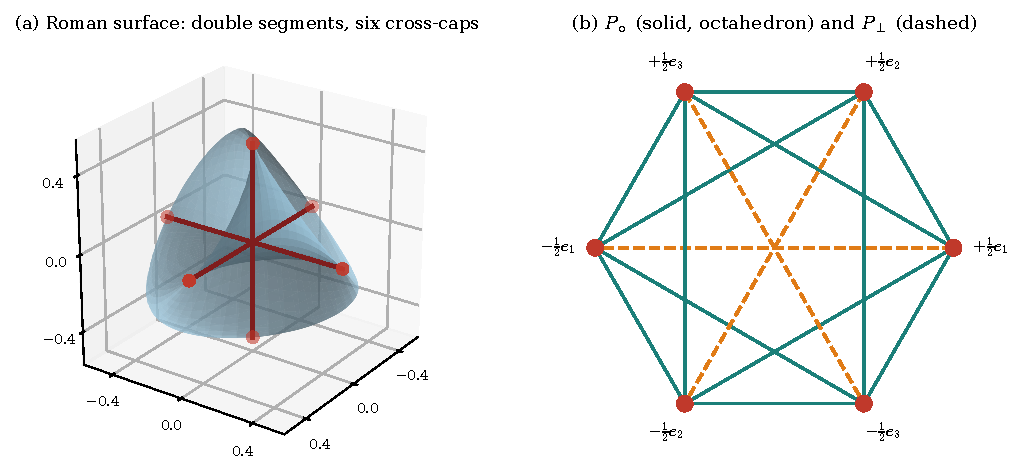
\includegraphics[width=\linewidth]{roman_surface.pdf}
\caption{(a) Steiner's Roman surface $f[x:y:z]=(yz,zx,xy)$. Its three double
segments (dark red) end at the six cross-caps $\pm\frac12e_k$. (b) The pair
structure of Theorem~\ref{thm:romanB}. The two ends of one double segment form
an orthogonal pair (dashed, the matrix $P_\perp$); all other pairs meet at
$60^\circ$ in the source and form the edges of an octahedron (solid, $P_\circ$).}\label{fig:roman}
\end{figure}

\begin{theorem}[Symmetry of the Green matrix]\label{thm:romanB}
Index the cross-caps so that $P_\perp$ pairs each with the unique one whose
line is orthogonal to it, and let $P_\circ=J-I-P_\perp$ be the adjacency of the
remaining pairs, whose lines meet at $60^\circ$. For every $\eta<0$ there are
real numbers $r,\gamma_\perp,\gamma_\circ$ with
\[
 B_\eta=r\,I+\gamma_\perp P_\perp+\gamma_\circ P_\circ .
\]
Hence $B_\eta$ has at most three eigenvalues: $r+\gamma_\perp+4\gamma_\circ$ on
the constants, $r+\gamma_\perp-2\gamma_\circ$ with multiplicity two, and
$r-\gamma_\perp$ with multiplicity three.
\end{theorem}
\begin{proof}
Each signed permutation $\sigma$ of coordinates descends to an isometry of
$(\mathbb{RP}^2,g)$, because $f\circ\sigma=L_\sigma\circ f$ for a signed
permutation $L_\sigma$ of $\R^3$, which is a Euclidean isometry. The pullback by
$\sigma$ is unitary, commutes with $H_F$ and $R_\eta$, permutes the cross-caps,
and preserves extrinsic radii. Hence it permutes the Green vectors, and
$(B_\eta)_{\sigma i\,\sigma j}=(B_\eta)_{ij}$. This group acts transitively on
the six cross-caps, and its orbits on ordered pairs of distinct cross-caps are
exactly the six orthogonal pairs and the twenty-four $60^\circ$ pairs
(verified). Symmetry of $B_\eta$ completes the form. $P_\perp$ and $P_\circ$
commute; $P_\circ$ is the adjacency matrix of the octahedron. Their joint
eigenvalues are $(1,4)$ on the constants, $(1,-2)$ on matching-even vectors of
sum zero, and $(-1,0)$ on matching-odd vectors.
\end{proof}

\subsection{A ruled surface with boundary cross-caps}\label{sec:ruled}

\begin{figure}[t]\centering
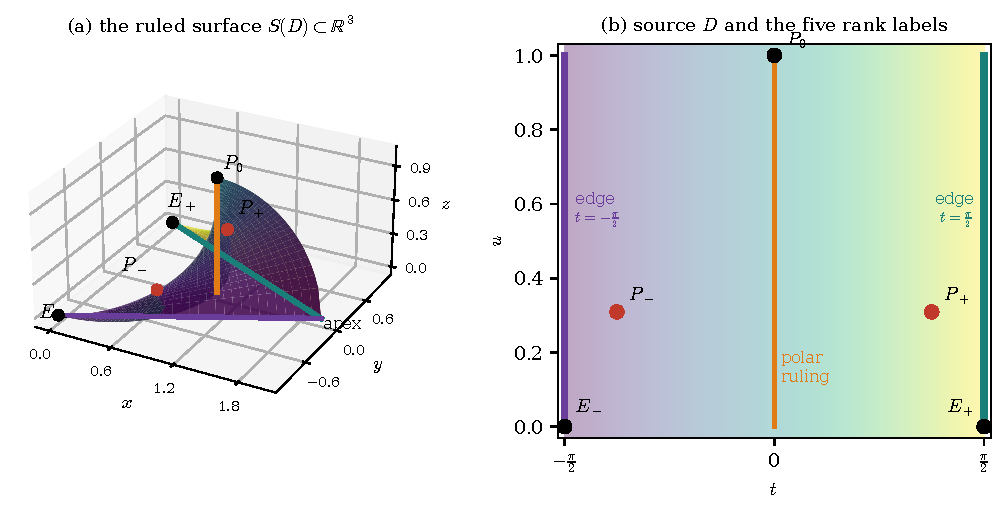
\includegraphics[width=\linewidth]{surface_overview.pdf}
\caption{The ruled surface of Section~\ref{sec:ruled} and its source. The
interior cross-caps $P_\pm$ carry the two logarithmic channels; $P_0$ is a
boundary half-germ and $E_\pm$ are corner quarter-germs, all on the
Dirichlet boundary.}\label{fig:ruled}
\end{figure}

The ruled map
\[
 S(t,u)=\bigl(\cos t+2u(1-\cos t),\,(1-u)\sin t,\,u\sqrt{\cos t(2-\cos t)}\bigr)
\]
on $[-\pi/2,\pi/2]\times[0,1]$, completed at $t=\pm\pi/2$ by the chart $r=Q$,
arose in a two-component signal model \cite{paper1,ruled}. It has five rank-one
points, all Whitney cross-caps \cite{ruled}. Two are interior:
$P_\pm=(\pm t_0,u_0)$ with $\cos t_0=(3-\sqrt5)/2$ and $u_0=(1-\cos t_0)/2$.
Three lie on the boundary: a half-germ at $(0,1)$ and two quarter-germs at
the lower corners. In the completed charts the boundary is formed by
coordinate lines, so Definition~\ref{def:setting} holds in case (D) with
$k=2$. All results apply. Moreover $S(-t,u)=JS(t,u)$ with
$J=\mathrm{diag}(1,-1,1)$ (Figure~\ref{fig:ruled}), and the argument of
Theorem~\ref{thm:romanB} shows
$B_\eta=\bigl(\begin{smallmatrix}r&\gamma\\\gamma&r\end{smallmatrix}\bigr)$. The Krein
extension has a two-dimensional kernel. An earlier preprint on this surface
\cite{record} defined the two-point problem through the compact-core closure
$H_0$ and claimed indices $(2,2)$; Proposition~\ref{prop:outer} shows why the
outer boundary must be fixed first.

\section{Open problems}\label{sec:open}
\begin{itemize}
\item \emph{Explicit regular parts.} Compute or estimate $B_\eta$, for instance
the three Roman-surface parameters, and relate them to global geometry.
\item \emph{Sharp local geometry.} For the standard germ $G-I=O(\rho\log(1/\rho))$
(Remark~\ref{rem:standard}). Is this the rate for every Whitney germ, and do
the Whitney invariants appear in the next term?
\item \emph{Spectral asymptotics.} By Corollary~\ref{cor:counting}, a Weyl
law for $H_F$ would hold for every extension. Establishing it for the
degenerate metric, and finding the heat-trace contribution of each cross-cap,
remain open.
\item \emph{Dirac operators.} A spinor or twisted Dirac analogue at cross-caps
needs closed domains, cut traces and transmission conditions. The
square-root monodromy of the observation field of the ruled surface suggests
a natural twist \cite{paper1}.
\item \emph{Other singularities.} Non-generic germs such as cuspidal edges or
$S_k^\pm$ singularities may carry different channel structures.
\end{itemize}

\appendix
\section{Evidence}\label{app:evidence}
The proofs above are given in full. The figures are generated by a script
from the explicit formulas of the paper; Figure~\ref{fig:euclidean} is a
numerical illustration of Remark~\ref{rem:standard}. The external inputs are the cross-cap
recognition criterion \cite{hasegawa}, Whitney's genericity theorem
\cite{whitney44,gg}, the scalar H\"older estimates \cite{gt,simon}, and the
abstract extension and Krein theorems \cite{pos,krein}. An exact replay checks
the algebra the proofs rely on: the adapted metric and determinant identities;
the explicit arclength coordinate of Remark~\ref{rem:standard} and its
derivative identities; the singular
set and Whitney determinants of the Roman surface; its symmetry orbits on pairs
of cross-caps; the eigenvalue pattern of $rI+\gamma_\perp P_\perp+\gamma_\circ P_\circ$;
and the reflection identity of the ruled surface. These checks do not certify
the analysis, and no Lean formalization of the analytic statements is claimed.
The verifier scripts and figure generator are archived in the software companion
\cite{software}, \href{https://doi.org/10.5281/zenodo.23103299}{doi:10.5281/zenodo.23103299}.

{\footnotesize
\begin{thebibliography}{99}
\bibitem{cdv} Y. Colin de Verdi\`ere, Pseudo-laplaciens I, \emph{Ann. Inst.
Fourier} 32 (1982), 275--286.
\bibitem{hk} L. Hillairet and A. Kokotov, Krein formula and $S$-matrix for
Euclidean surfaces with conical singularities, \emph{J. Geom. Anal.} 23 (2013),
1498--1529;
\href{https://arxiv.org/abs/1011.5034}{arXiv:1011.5034}.
\bibitem{grieser} D. Grieser, Quasiisometry of singular metrics, \emph{Houston
J. Math.} 28 (2002), 741--752.
\bibitem{whitney44} H. Whitney, The singularities of a smooth $n$-manifold in
$(2n-1)$-space, \emph{Ann. of Math.} 45 (1944), 247--293.
\bibitem{gg} M. Golubitsky and V. Guillemin, \emph{Stable Mappings and Their
Singularities}, Springer, 1973.
\bibitem{hasegawa} M. Hasegawa et al., Intrinsic properties of surfaces with
singularities, \href{https://arxiv.org/abs/1409.0281}{arXiv:1409.0281}, \S4.
\bibitem{pos} A. Posilicano, Boundary triples and Weyl functions for singular
perturbations of self-adjoint operators, \emph{Methods Funct. Anal. Topology}
10 (2004), 57--63; \href{https://arxiv.org/abs/math/0309077}{arXiv:math/0309077}.
\bibitem{gt} D. Gilbarg and N. S. Trudinger, \emph{Elliptic Partial
Differential Equations of Second Order}, Springer, Thm.~8.24.
\bibitem{simon} L. Simon, Lectures on PDE, Lecture 18, Theorems 2--3,
\url{https://math.stanford.edu/~lms/lecs-on-pde.pdf}.
\bibitem{krein} M. S. Ashbaugh, F. Gesztesy, M. Mitrea, R. Shterenberg and
G. Teschl, The Krein--von Neumann extension and its connection to an abstract
buckling problem, \href{https://arxiv.org/abs/0907.1439}{arXiv:0907.1439}.
\bibitem{abr} S. Albeverio, J. Brasche and M. R\"ockner, Dirichlet forms and
generalized Schr\"odinger operators, in \emph{Schr\"odinger Operators}, Lecture
Notes in Physics 345, Springer, 1989.
\bibitem{ruled} A. Hayami, The Orthogonal-Circle Ruled Surface, 2026,
\href{https://doi.org/10.5281/zenodo.23073642}{doi:10.5281/zenodo.23073642}.
\bibitem{paper1} A. Hayami, Realization Limits of the Bicomplex Signal Surface:
Analytic Rigidity, Smooth Flexibility and Observation Monodromy, preprint, Zenodo,
2026, \href{https://doi.org/10.5281/zenodo.23103026}{doi:10.5281/zenodo.23103026}.
\bibitem{software} A. Hayami, Verification Companion for Realization Limits and
Pseudo-Laplacians at Whitney Cross-Caps, software, Zenodo, 2026,
\href{https://doi.org/10.5281/zenodo.23103299}{doi:10.5281/zenodo.23103299}.
\bibitem{record} A. Hayami (J.-Y. Huang), Geometric Realization of Bicomplex
Signal Manifolds, preprint, ResearchGate, 2026,
\href{https://doi.org/10.13140/RG.2.2.17048.15361}{doi:10.13140/RG.2.2.17048.15361}.
\end{thebibliography}}
\end{document}
